\documentclass[../Bachelorarbeit.tex]{subfiles}

\begin{document}
\label{sec:BSM}
\begin{figure}
    \centering
    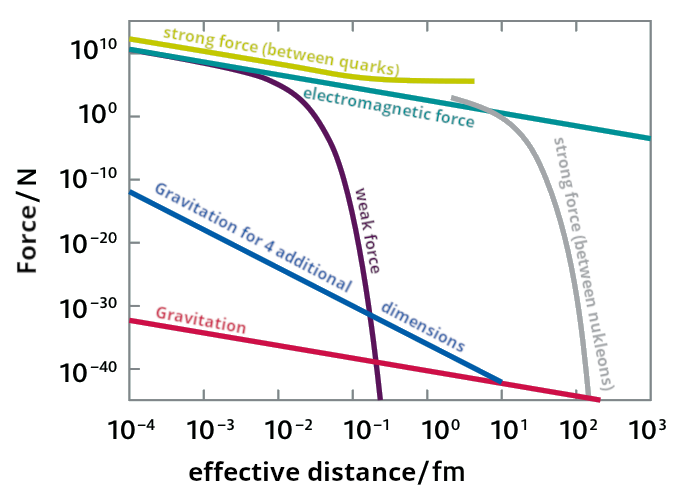
\includegraphics[width=0.5\textwidth]{images/Teilchenwet_WW_range.png}
    \caption{Interaction strength for different ranges of the Fundamental interactions. Although the Nuclear force isn't a fundamental it is shown in order to visualize point (c). Translation of the interaction }
    \label{fig:WW_range}
\end{figure}

In 2012 the last particle predicted by the SM was detected at CERN the Higgs Boson. Yet again proving the success of the SM.
But this also means no more free parameters in the SM for new particles. All interactions found obey the local $SU(3) \times SU(2) \times U(1)$ gauge symmetries
and later data only strengthens the SM prediction. While no data was found suggesting inconsistencies with the electroweak symmetry breaking $SU(2) \times U(1) \rightarrow U(1)$
and no new exotic particles are found between 0-2 TeV \ref{fig:ATLAS_SUSY}.
This means physicist have to search for new interactions considering different interaction ranges and strengths(Figure \ref{fig:WW_range}).
\begin{enumerate}[label=(\alph*)]
    \item Considerably weaker than gravitation with infinite range
    \item Shorter range than the weak interaction of any strength
    \item Range between weak interaction and nuclear force and considerably weaker than the weak interaction 
\end{enumerate}

There are various methods for finding BSM particles and as many theoretical models for new interactions, but these can generally be broken down in three categories.
\\\\
The Model specific search where one takes a well-defined model often describing a complete UV theory and try's to find the predicted particles in measurements.
The most popular example for this is the Supersymmetry(SUSY) which is often associated with the search for Dark Matter and adds a wide range of different particles.
In the search for Dark Matter one would look for example look for missing transverse momentum in top quark interactions or look for resonance with the so-called
two Higgs doublet models.
\\\\
Another way of looking for new physics is by using simplified Models. Here one takes a well-defined model in order to describe some aspects or specific phenomenon of the UV Theory.
Again a good example comes from dark matter physics the beautifully named neutralino in Minimale Supersymmetry Standard Model(MSSM) with MSSM being a low energy model of the SUSY.
Here the for neutralinos are electrically neutral fermions with a mass over 300 GeV and conserves the hypothetical R-parity in MSSM. Compared to the Model specific search the result
would give evidence only for the R-partiy and the neutralino but not for other aspects of SUSY.
\\\\
These first two methods depend entirely on a theoretical model. Granted these models are often well motivated by known physics or mathematical structures.
But history has shown multiple times that experiments can produce unexpected results. As a recent example being the accelerating expansion of the Universe by some so-called Dark Energy.
Unfortunately unexpected results are often not described by existing models, therefore a model independent search has to be done and EFT is the primary tool for this in particle physics.
Taking a look at the Fermi Theory (section \ref{sec:Fermi}) again one will realize that Fermi's Theory was able to approximate the weak interaction but isn't able to describe the
structure of weak interactions. Only using Fermi's Theory one would not be able to describe CP-Violation. Generally describing an exotic interaction using EFT one can only predict low order
processes, but the low energy observer can't make predicting as to what he is actually describing. The results can then be used to construct an appropriate model or match an existing one and
use the first to methods to validate this model.

\begin{figure}
    \centering
    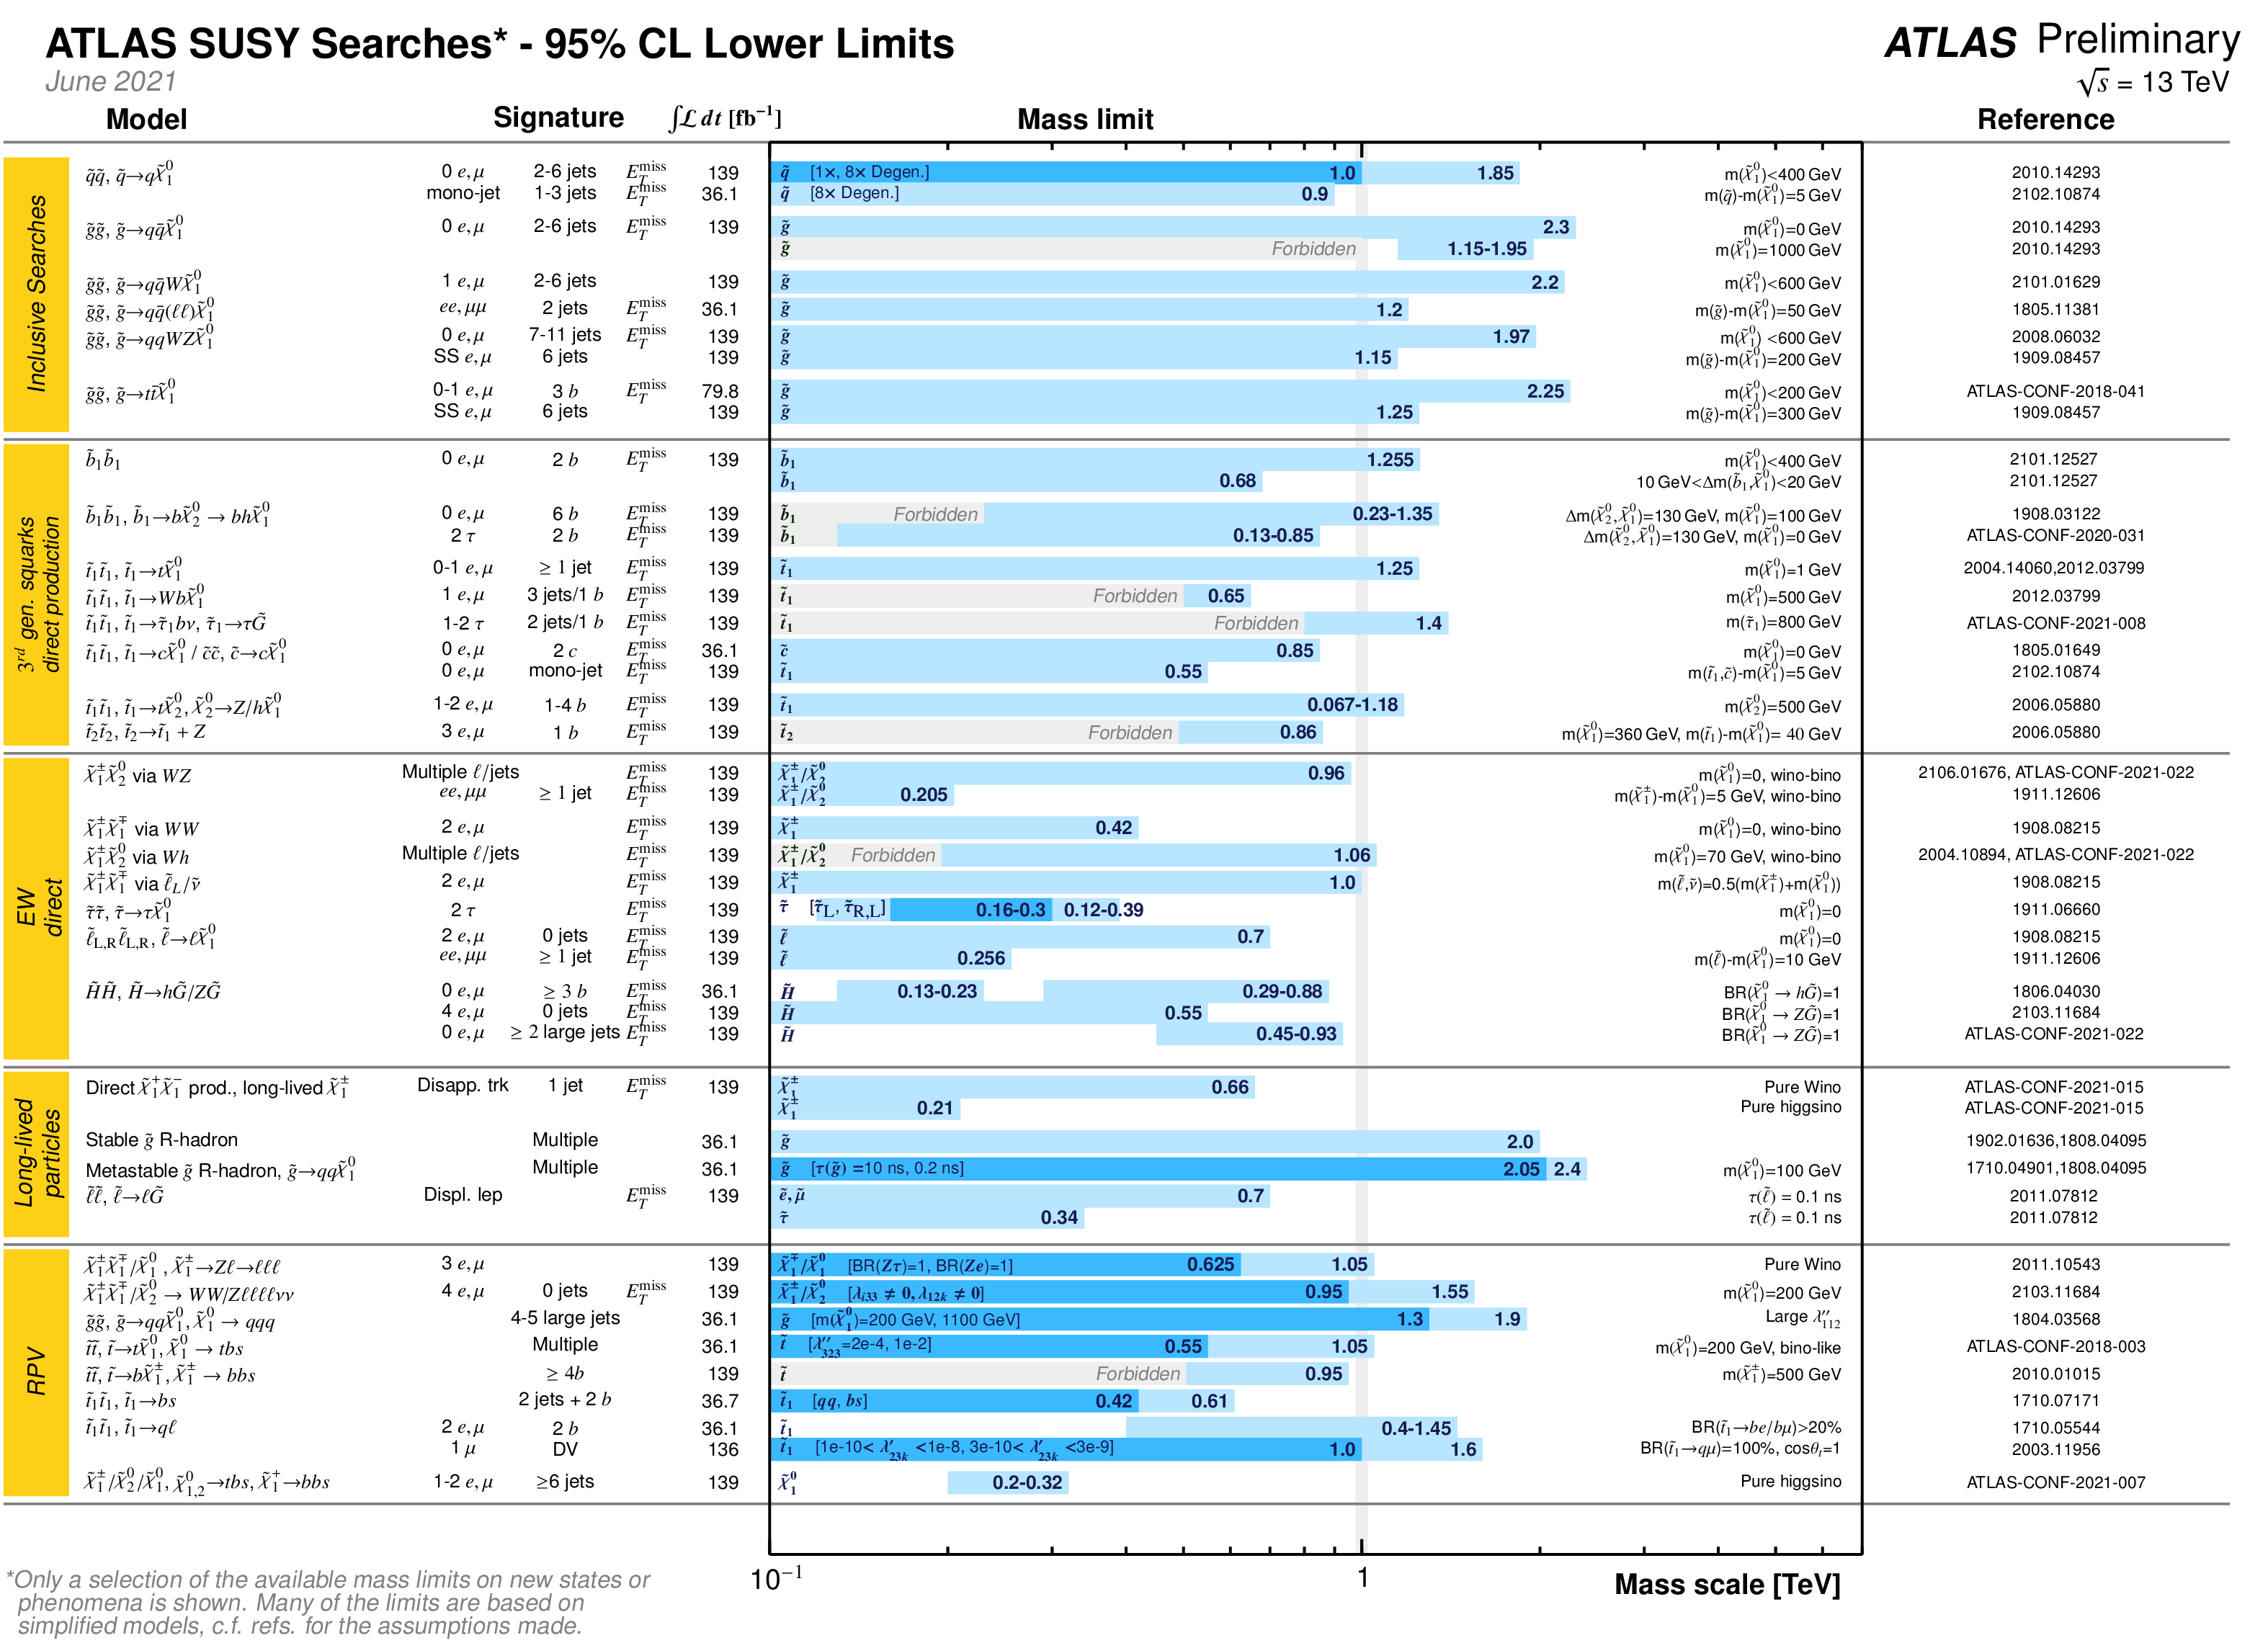
\includegraphics[width=0.5\textwidth]{images/fig_23_ATLAS_SUSY.png}
    \caption{ASK what this is \cite{.07.06.2021}}
    \label{fig:ATLAS_SUSY}
\end{figure}

\end{document}